\documentclass[tikz, border=0pt]{standalone}
\usepackage{siunitx}
\usepackage{physics}
\usepackage{amsmath}
\usetikzlibrary{decorations,decorations.markings,decorations.text,decorations.pathreplacing}
\usetikzlibrary{matrix,positioning,fit,backgrounds,intersections}
\usetikzlibrary{arrows.meta}
\usetikzlibrary{calc}

\definecolor{amber}{rgb}{1.0, 0.75, 0.0}
\definecolor{goldmetallic}{rgb}{0.83, 0.69, 0.22}
\definecolor{airforceblue}{rgb}{0.36, 0.54, 0.66}  %#5D8AA8
\definecolor{cobalt}{rgb}{0.0, 0.28, 0.67}         %#0047AB
\definecolor{coolblack}{rgb}{0.0, 0.18, 0.39}      %#002E63
\definecolor{dartmouthgreen}{rgb}{0.05, 0.5, 0.06} %#00693E
\definecolor{mydmg}{rgb}{0.05, 0.5, 0.06}          %#00693E
\definecolor{lava}{rgb}{0.81, 0.06, 0.13}          %#CF1020
\definecolor{myred}{rgb}{0.81, 0.06, 0.13}         %#CF1020


\makeatletter
\DeclareRobustCommand{\rvdots}{%
  \vbox{
    \baselineskip4\p@\lineskiplimit\z@
    \kern-\p@
    \hbox{.}\hbox{.}\hbox{.}
  }}
\makeatother


\begin{document}


\def\layersep{1.0cm}
%\begin{minipage}{0.6\columnwidth}
    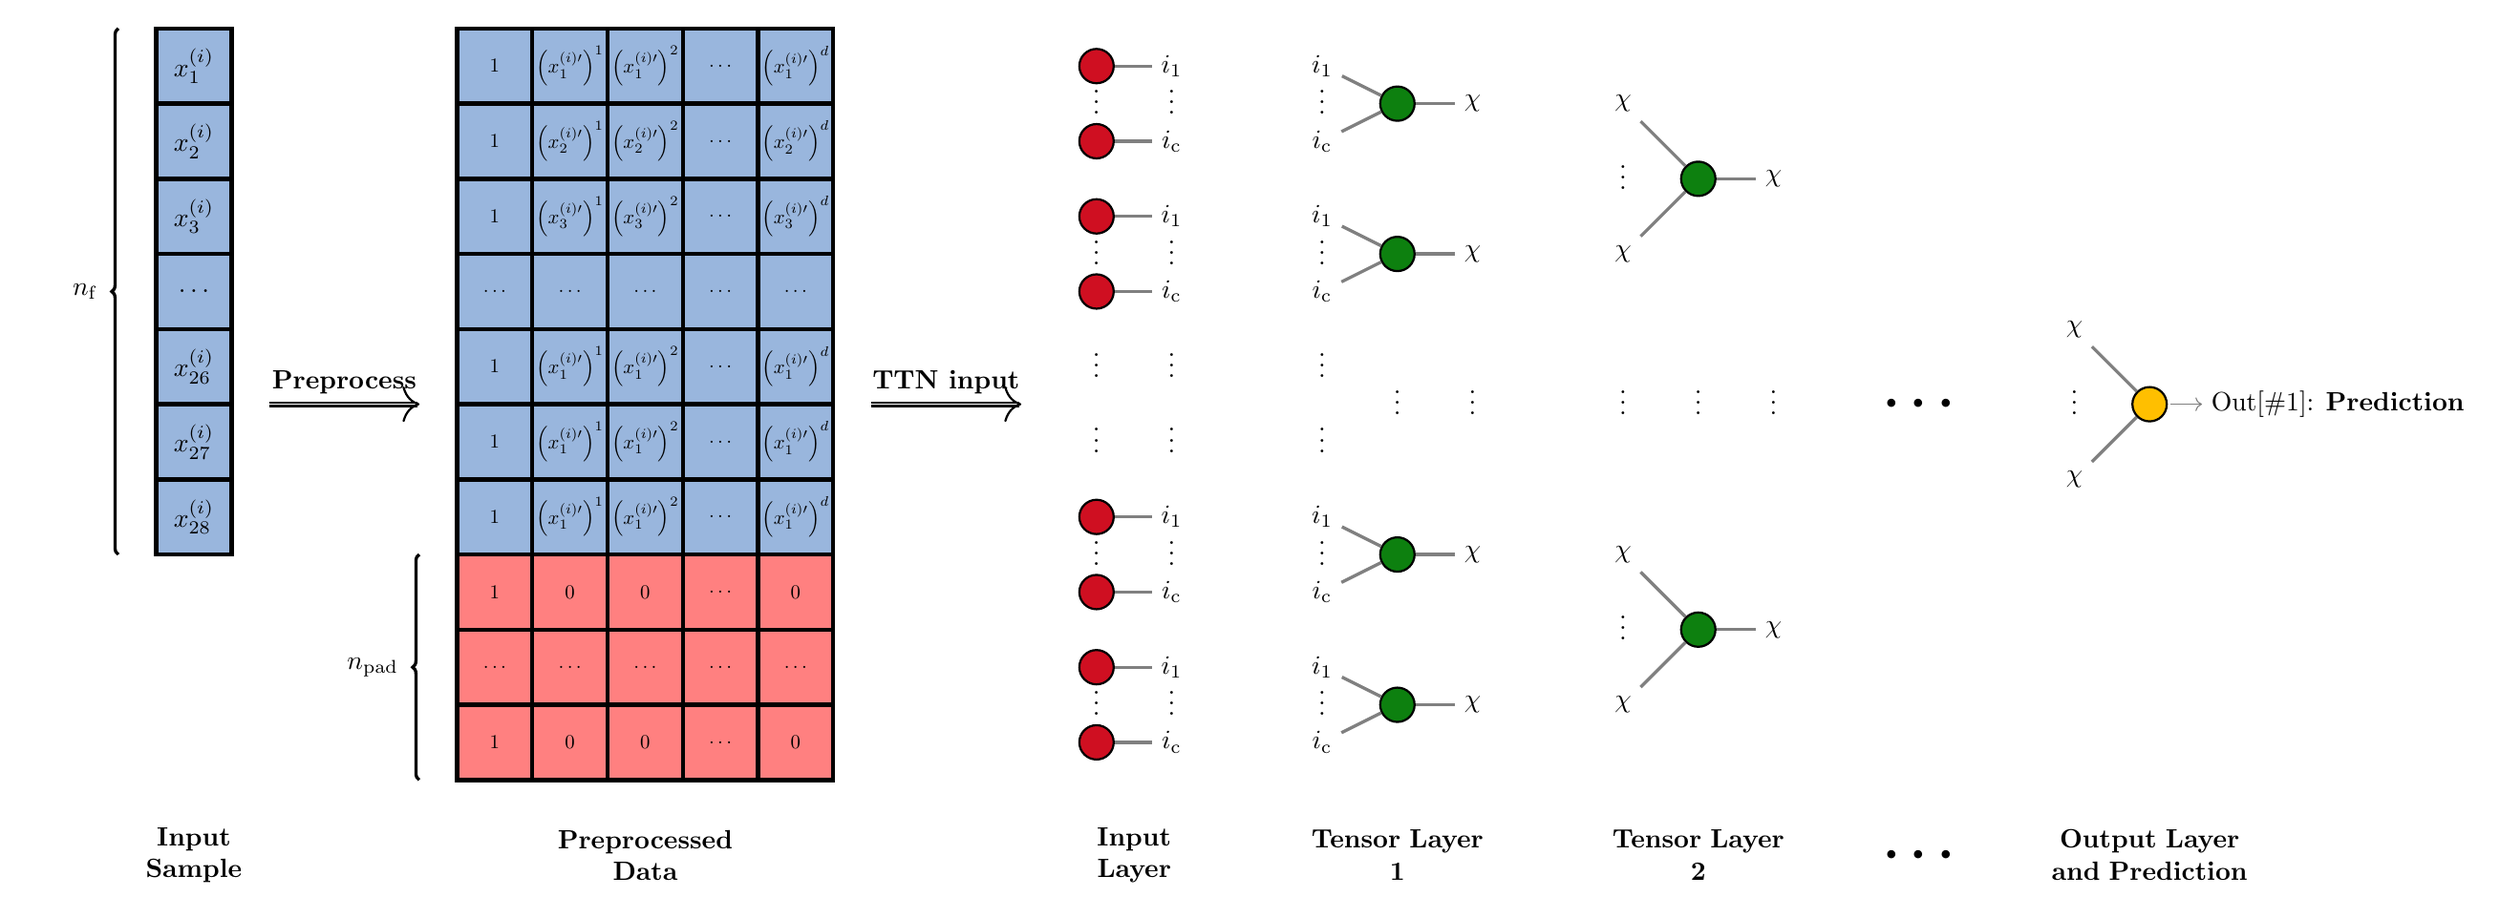
\begin{tikzpicture}[
        draw=black!50,
        node distance=0.3em,
        transform shape,scale=1.0
    ]
    
    \tikzstyle{annot} = [text width=12em, text centered]
    
    \def\XPA{0}
    \def\XPB{4}
    \def\XPC{8}
    \def\XPD{4}
    
    % upper
    \draw[ultra thick, draw=black, fill=white!60!cobalt] (\XPA,0) grid (\XPA+1,- 7) rectangle (\XPA,0);
    % \draw[ultra thick, draw=black, fill=white!60!cobalt] (\XPB,0) grid (\XPB+1,- 7) rectangle (\XPB,0);
    % \draw[ultra thick, draw=black, fill=white!60!cobalt] (\XPC,0) grid (\XPC+1,- 7) rectangle (\XPC,0);
    \draw[ultra thick, draw=black, fill=white!60!cobalt] (\XPD,0) grid (\XPD+5,- 7) rectangle (\XPD,0);
    
    % pad
    % \draw[ultra thick, draw=black, fill=white!50!red] (\XPC,-7) grid (\XPC+1,-10) rectangle (\XPC,-7);
    \draw[ultra thick, draw=black, fill=white!50!red] (\XPD,-7) grid (\XPD+5,-10) rectangle (\XPD,-7);
    
    % PA nodes
    \node (PA-1)  at (\XPA+0.5,- 0.5) {\( x^{(i)}_{1}  \)};
    \node (PA-2)  at (\XPA+0.5,- 1.5) {\( x^{(i)}_{2}  \)};
    \node (PA-3)  at (\XPA+0.5,- 2.5) {\( x^{(i)}_{3}  \)};
    \node (PA-D)  at (\XPA+0.5,- 3.5) {\( \dots  \)};
    \node (PA-26) at (\XPA+0.5,- 4.5) {\( x^{(i)}_{26} \)};
    \node (PA-27) at (\XPA+0.5,- 5.5) {\( x^{(i)}_{27} \)};
    \node (PA-28) at (\XPA+0.5,- 6.5) {\( x^{(i)}_{28} \)};
    
    % PB nodes
    % \node (PB-1)  at (\XPB+0.5,- 0.5) {\( x^{(i)\prime}_{1}  \)};
    % \node (PB-2)  at (\XPB+0.5,- 1.5) {\( x^{(i)\prime}_{2}  \)};
    % \node (PB-3)  at (\XPB+0.5,- 2.5) {\( x^{(i)\prime}_{3}  \)};
    % \node (PB-D)  at (\XPB+0.5,- 3.5) {\( \dots              \)};
    % \node (PB-26) at (\XPB+0.5,- 4.5) {\( x^{(i)\prime}_{26} \)};
    % \node (PB-27) at (\XPB+0.5,- 5.5) {\( x^{(i)\prime}_{27} \)};
    % \node (PB-28) at (\XPB+0.5,- 6.5) {\( x^{(i)\prime}_{28} \)};
    
    % PC nodes
    % \node (PC-1)  at (\XPC+0.5,- 0.5) {\( x^{(i)\prime}_{1}  \)};
    % \node (PC-2)  at (\XPC+0.5,- 1.5) {\( x^{(i)\prime}_{2}  \)};
    % \node (PC-3)  at (\XPC+0.5,- 2.5) {\( x^{(i)\prime}_{3}  \)};
    % \node (PC-D)  at (\XPC+0.5,- 3.5) {\( \dots              \)};
    % \node (PC-26) at (\XPC+0.5,- 4.5) {\( x^{(i)\prime}_{26} \)};
    % \node (PC-27) at (\XPC+0.5,- 5.5) {\( x^{(i)\prime}_{27} \)};
    % \node (PC-28) at (\XPC+0.5,- 6.5) {\( x^{(i)\prime}_{28} \)};
    % \node (PC-P1) at (\XPC+0.5,- 7.5) {\( 0                  \)};
    % \node (PC-PD) at (\XPC+0.5,- 8.5) {\( \dots              \)};
    % \node (PC-P3) at (\XPC+0.5,- 9.5) {\( 0                  \)};
    
    % PD nodes
    \node[scale=0.75] (PD0-1)  at (\XPD+0.5,- 0.5) {\( 1     \)};
    \node[scale=0.75] (PD0-2)  at (\XPD+0.5,- 1.5) {\( 1     \)};
    \node[scale=0.75] (PD0-3)  at (\XPD+0.5,- 2.5) {\( 1     \)};
    \node[scale=0.75] (PD0-D)  at (\XPD+0.5,- 3.5) {\( \dots \)};
    \node[scale=0.75] (PD0-26) at (\XPD+0.5,- 4.5) {\( 1     \)};
    \node[scale=0.75] (PD0-27) at (\XPD+0.5,- 5.5) {\( 1     \)};
    \node[scale=0.75] (PD0-28) at (\XPD+0.5,- 6.5) {\( 1     \)};
    \node[scale=0.75] (PD0-P1) at (\XPD+0.5,- 7.5) {\( 1     \)};
    \node[scale=0.75] (PD0-PD) at (\XPD+0.5,- 8.5) {\( \dots \)};
    \node[scale=0.75] (PD0-P3) at (\XPD+0.5,- 9.5) {\( 1     \)};
    %%% PD1 nodes
    \node[scale=0.75] (PD1-1)  at (\XPD+1.5,- 0.5) {\( \qty(x^{(i)\prime}_{1})^{1}  \)};
    \node[scale=0.75] (PD1-2)  at (\XPD+1.5,- 1.5) {\( \qty(x^{(i)\prime}_{2})^{1}  \)};
    \node[scale=0.75] (PD1-3)  at (\XPD+1.5,- 2.5) {\( \qty(x^{(i)\prime}_{3})^{1}  \)};
    \node[scale=0.75] (PD1-D)  at (\XPD+1.5,- 3.5) {\( \dots                        \)};
    \node[scale=0.75] (PD1-26) at (\XPD+1.5,- 4.5) {\( \qty(x^{(i)\prime}_{1})^{1}  \)};
    \node[scale=0.75] (PD1-27) at (\XPD+1.5,- 5.5) {\( \qty(x^{(i)\prime}_{1})^{1}  \)};
    \node[scale=0.75] (PD1-28) at (\XPD+1.5,- 6.5) {\( \qty(x^{(i)\prime}_{1})^{1}  \)};
    \node[scale=0.75] (PD1-P1) at (\XPD+1.5,- 7.5) {\( 0                            \)};
    \node[scale=0.75] (PD1-PD) at (\XPD+1.5,- 8.5) {\( \dots                        \)};
    \node[scale=0.75] (PD1-P3) at (\XPD+1.5,- 9.5) {\( 0                            \)};
    %%% PD2 nodes
    \node[scale=0.75] (PD2-1)  at (\XPD+2.5,- 0.5) {\( \qty(x^{(i)\prime}_{1})^{2}  \)};
    \node[scale=0.75] (PD2-2)  at (\XPD+2.5,- 1.5) {\( \qty(x^{(i)\prime}_{2})^{2}  \)};
    \node[scale=0.75] (PD2-3)  at (\XPD+2.5,- 2.5) {\( \qty(x^{(i)\prime}_{3})^{2}  \)};
    \node[scale=0.75] (PD2-D)  at (\XPD+2.5,- 3.5) {\( \dots                        \)};
    \node[scale=0.75] (PD2-26) at (\XPD+2.5,- 4.5) {\( \qty(x^{(i)\prime}_{1})^{2}  \)};
    \node[scale=0.75] (PD2-27) at (\XPD+2.5,- 5.5) {\( \qty(x^{(i)\prime}_{1})^{2}  \)};
    \node[scale=0.75] (PD2-28) at (\XPD+2.5,- 6.5) {\( \qty(x^{(i)\prime}_{1})^{2}  \)};
    \node[scale=0.75] (PD2-P1) at (\XPD+2.5,- 7.5) {\( 0                            \)};
    \node[scale=0.75] (PD2-PD) at (\XPD+2.5,- 8.5) {\( \dots                        \)};
    \node[scale=0.75] (PD2-P3) at (\XPD+2.5,- 9.5) {\( 0                            \)};
    %%% PD dots nodes
    \node[scale=0.75] (PD-D) at (\XPD+3.5,- 0.5) {\( \dots \)};
    \node[scale=0.75] (PD-D) at (\XPD+3.5,- 1.5) {\( \dots \)};
    \node[scale=0.75] (PD-D) at (\XPD+3.5,- 2.5) {\( \dots \)};
    \node[scale=0.75] (PD-D) at (\XPD+3.5,- 3.5) {\( \dots \)};
    \node[scale=0.75] (PD-D) at (\XPD+3.5,- 4.5) {\( \dots \)};
    \node[scale=0.75] (PD-D) at (\XPD+3.5,- 5.5) {\( \dots \)};
    \node[scale=0.75] (PD-D) at (\XPD+3.5,- 6.5) {\( \dots \)};
    \node[scale=0.75] (PD-D) at (\XPD+3.5,- 7.5) {\( \dots \)};
    \node[scale=0.75] (PD-D) at (\XPD+3.5,- 8.5) {\( \dots \)};
    \node[scale=0.75] (PD-D) at (\XPD+3.5,- 9.5) {\( \dots \)};
    %%% PDD nodes
    \node[scale=0.75] (PDD-1)  at (\XPD+4.5,- 0.5) {\( \qty(x^{(i)\prime}_{1})^{d}  \)};
    \node[scale=0.75] (PDD-2)  at (\XPD+4.5,- 1.5) {\( \qty(x^{(i)\prime}_{2})^{d}  \)};
    \node[scale=0.75] (PDD-3)  at (\XPD+4.5,- 2.5) {\( \qty(x^{(i)\prime}_{3})^{d}  \)};
    \node[scale=0.75] (PDD-D)  at (\XPD+4.5,- 3.5) {\( \dots                        \)};
    \node[scale=0.75] (PDD-26) at (\XPD+4.5,- 4.5) {\( \qty(x^{(i)\prime}_{1})^{d}  \)};
    \node[scale=0.75] (PDD-27) at (\XPD+4.5,- 5.5) {\( \qty(x^{(i)\prime}_{1})^{d}  \)};
    \node[scale=0.75] (PDD-28) at (\XPD+4.5,- 6.5) {\( \qty(x^{(i)\prime}_{1})^{d}  \)};
    \node[scale=0.75] (PDD-P1) at (\XPD+4.5,- 7.5) {\( 0                            \)};
    \node[scale=0.75] (PDD-PD) at (\XPD+4.5,- 8.5) {\( \dots                        \)};
    \node[scale=0.75] (PDD-P3) at (\XPD+4.5,- 9.5) {\( 0                            \)};
    
    % PA->PB
    \draw[double,->, thick, black] (\XPA+1.5, -5.0) -- (\XPD-0.5, -5.0) node[midway, anchor=south, align=center] {\textbf{Preprocess}};
    
    % PB->PC
    % \draw[double,->, thick, black] (\XPB+1.5, -5.0) -- (\XPC-0.5, -5.0) node[midway, anchor=south, align=center] {\textbf{Zero pad}};
    
    % PC->PD
    % \draw[double,->, thick, black] (\XPC+1.5, -5.0) -- (\XPD-0.5, -5.0) node[midway, anchor=south, align=center] {\textbf{Map}};
    
    
    % underbraces
    \draw[
        very thick,
        decoration={
            brace,
            mirror,
            raise=0.1
        },
        decorate,
        black
    ] (\XPA-0.5,0) -- (\XPA-0.5,-7) node [midway, anchor=west, xshift=-0.75cm] {\( n_{\mathrm{f}} \)};
    
    \draw[
        very thick,
        decoration={
            brace,
            mirror,
            raise=0.1
        },
        decorate,
        black
    ] (\XPD-0.5,-7) -- (\XPD-0.5,-10) node [midway, anchor=west, xshift=-1.1cm] {\( n_{\mathrm{pad}} \)};
    
    
    % annotations
    \node[annot, below of=PA-28, node distance=4.5cm]  (PA-TEXT) {\textbf{Input\\Sample}};
    % \node[annot, below of=PB-28, node distance=4.5cm]  (PB-TEXT) {\textbf{Rescaling in\\\( \boldsymbol{[0,1]} \) or \( \boldsymbol{[-1,1]} \)}};
    % \node[annot, below of=PC-28, node distance=4.5cm]  (PC-TEXT) {\textbf{Zero\\Padding}};
    \node[annot, below of=PD2-28, node distance=4.5cm] (PC-TEXT) {\textbf{Preprocessed\\Data}};
    
    
    
    
    
    \tikzstyle{every pin edge}=[<-,shorten <=1pt]
    \tikzstyle{neuron}=[circle,fill=black!25,minimum size=13pt,inner sep=0pt]
    \tikzstyle{input neuron}=[neuron, fill=lava];
    \tikzstyle{output neuron}=[neuron, fill=amber];
    \tikzstyle{hidden neuron}=[neuron, fill=dartmouthgreen];
    
    \def\XTA{20-8}
    \def\XTB{21-8}
    \def\XTC{23-8}
    \def\XTD{24-8}
    \def\XTE{25-8}
    \def\XTF{27-8}
    \def\XTG{28-8}
    \def\XTH{29-8}
    \def\XTI{31-8}
    \def\XTJ{33-8}
    \def\XTK{34-8}
    \def\XTL{35-8}
    
    % input nodes
    \node[input neuron, draw=black!100, thick] (TA-1)  at (\XTA+0.5,- 0.5) {};
    \node[scale=1.00, anchor=center]           (TA-D1) at (\XTA+0.5,- 1.0) {\( \boldsymbol{\rvdots} \)};
    \node[input neuron, draw=black!100, thick] (TA-2)  at (\XTA+0.5,- 1.5) {};
    \node[input neuron, draw=black!100, thick] (TA-3)  at (\XTA+0.5,- 2.5) {};
    \node[scale=1.00, anchor=center]           (TA-D2) at (\XTA+0.5,- 3.0) {\( \boldsymbol{\rvdots} \)};
    \node[input neuron, draw=black!100, thick] (TA-4)  at (\XTA+0.5,- 3.5) {};
    \node[scale=1.00, anchor=center]           (TA-D3) at (\XTA+0.5,- 4.5) {\( \boldsymbol{\rvdots} \)};
    \node[scale=1.00, anchor=center]           (TA-D4) at (\XTA+0.5,- 5.5) {\( \boldsymbol{\rvdots} \)};
    \node[input neuron, draw=black!100, thick] (TA-7)  at (\XTA+0.5,- 6.5) {};
    \node[scale=1.00, anchor=center]           (TA-D5) at (\XTA+0.5,- 7.0) {\( \boldsymbol{\rvdots} \)};
    \node[input neuron, draw=black!100, thick] (TA-8)  at (\XTA+0.5,- 7.5) {};
    \node[input neuron, draw=black!100, thick] (TA-9)  at (\XTA+0.5,- 8.5) {};
    \node[scale=1.00, anchor=center]           (TA-D6) at (\XTA+0.5,- 9.0) {\( \boldsymbol{\rvdots} \)};
    \node[input neuron, draw=black!100, thick] (TA-10) at (\XTA+0.5,- 9.5) {};
    
    % input edges nodes
    \node[scale=1.00, anchor=center] (TB-1)  at (\XTB+0.5,- 0.5) {\( i_{1}                \)};
    \node[scale=1.00, anchor=center] (TB-D1) at (\XTB+0.5,- 1.0) {\( \boldsymbol{\rvdots} \)};
    \node[scale=1.00, anchor=center] (TB-2)  at (\XTB+0.5,- 1.5) {\( i_{\mathrm{c}}       \)};
    \node[scale=1.00, anchor=center] (TB-3)  at (\XTB+0.5,- 2.5) {\( i_{1}                \)};
    \node[scale=1.00, anchor=center] (TB-D2) at (\XTB+0.5,- 3.0) {\( \boldsymbol{\rvdots} \)};
    \node[scale=1.00, anchor=center] (TB-4)  at (\XTB+0.5,- 3.5) {\( i_{\mathrm{c}}       \)};
    \node[scale=1.00, anchor=center] (TB-D3) at (\XTB+0.5,- 4.5) {\( \boldsymbol{\rvdots} \)};
    \node[scale=1.00, anchor=center] (TB-D4) at (\XTB+0.5,- 5.5) {\( \boldsymbol{\rvdots} \)};
    \node[scale=1.00, anchor=center] (TB-7)  at (\XTB+0.5,- 6.5) {\( i_{1}                \)};
    \node[scale=1.00, anchor=center] (TB-D5) at (\XTB+0.5,- 7.0) {\( \boldsymbol{\rvdots} \)};
    \node[scale=1.00, anchor=center] (TB-8)  at (\XTB+0.5,- 7.5) {\( i_{\mathrm{c}}       \)};
    \node[scale=1.00, anchor=center] (TB-9)  at (\XTB+0.5,- 8.5) {\( i_{1}                \)};
    \node[scale=1.00, anchor=center] (TB-D6) at (\XTB+0.5,- 9.0) {\( \boldsymbol{\rvdots} \)};
    \node[scale=1.00, anchor=center] (TB-10) at (\XTB+0.5,- 9.5) {\( i_{\mathrm{c}}       \)};
    
    % input edges
    \draw[very thick] (TA-1)  -- (TB-1) ;
    % \draw[thick] (TA-D1) -- (TB-D1);
    \draw[very thick] (TA-2)  -- (TB-2) ;
    \draw[very thick] (TA-3)  -- (TB-3) ;
    % \draw[thick] (TA-D2) -- (TB-D2);
    \draw[very thick] (TA-4)  -- (TB-4) ;
    % \draw[thick] (TA-D3) -- (TB-D3);
    % \draw[thick] (TA-D4) -- (TB-D4);
    \draw[very thick] (TA-7)  -- (TB-7) ;
    % \draw[thick] (TA-D5) -- (TB-D5);
    \draw[very thick] (TA-8)  -- (TB-8) ;
    \draw[very thick] (TA-9)  -- (TB-9) ;
    % \draw[thick] (TA-D6) -- (TB-D6);
    \draw[very thick] (TA-10) -- (TB-10);
    
    % output edges nodes 1
    \node[scale=1.00, anchor=center] (TC-1)  at (\XTC+0.5,- 0.5) {\( i_{1}                \)};
    \node[scale=1.00, anchor=center] (TC-D1) at (\XTC+0.5,- 1.0) {\( \boldsymbol{\rvdots} \)};
    \node[scale=1.00, anchor=center] (TC-2)  at (\XTC+0.5,- 1.5) {\( i_{\mathrm{c}}       \)};
    \node[scale=1.00, anchor=center] (TC-3)  at (\XTC+0.5,- 2.5) {\( i_{1}                \)};
    \node[scale=1.00, anchor=center] (TC-D2) at (\XTC+0.5,- 3.0) {\( \boldsymbol{\rvdots} \)};
    \node[scale=1.00, anchor=center] (TC-4)  at (\XTC+0.5,- 3.5) {\( i_{\mathrm{c}}       \)};
    \node[scale=1.00, anchor=center] (TC-D3) at (\XTC+0.5,- 4.5) {\( \boldsymbol{\rvdots} \)};
    \node[scale=1.00, anchor=center] (TC-D4) at (\XTC+0.5,- 5.5) {\( \boldsymbol{\rvdots} \)};
    \node[scale=1.00, anchor=center] (TC-7)  at (\XTC+0.5,- 6.5) {\( i_{1}                \)};
    \node[scale=1.00, anchor=center] (TC-D5) at (\XTC+0.5,- 7.0) {\( \boldsymbol{\rvdots} \)};
    \node[scale=1.00, anchor=center] (TC-8)  at (\XTC+0.5,- 7.5) {\( i_{\mathrm{c}}       \)};
    \node[scale=1.00, anchor=center] (TC-9)  at (\XTC+0.5,- 8.5) {\( i_{1}                \)};
    \node[scale=1.00, anchor=center] (TC-D6) at (\XTC+0.5,- 9.0) {\( \boldsymbol{\rvdots} \)};
    \node[scale=1.00, anchor=center] (TC-10) at (\XTC+0.5,- 9.5) {\( i_{\mathrm{c}}       \)};
    
    % output edges nodes 1
    \node[hidden neuron, draw=black!100, thick, anchor=center] (TD-1) at (\XTD+0.5,- 1.0) {};
    % \node[hidden neuron, draw=black!100, thick, anchor=center] (TD-3)  at (\XTD+0.5,- 2.5) {};
    \node[hidden neuron, draw=black!100, thick, anchor=center] (TD-2) at (\XTD+0.5,- 3.0) {};
    % \node[hidden neuron, draw=black!100, thick, anchor=center] (TD-4)  at (\XTD+0.5,- 3.5) {};
    % \node[hidden neuron, draw=black!100, thick, anchor=center] (TD-D3) at (\XTD+0.5,- 4.5) {\( \boldsymbol{\rvdots} \)};
    % \node[hidden neuron, draw=black!100, thick, anchor=center] (TD-D4) at (\XTD+0.5,- 5.5) {\( \boldsymbol{\rvdots} \)};
    % \node[hidden neuron, draw=black!100, thick, anchor=center] (TD-7)  at (\XTD+0.5,- 6.5) {};
    \node[scale=1.00, anchor=center] (TD-D1) at (\XTD+0.5,- 5.0) {\( \boldsymbol{\rvdots} \)};
    \node[hidden neuron, draw=black!100, thick, anchor=center] (TD-3) at (\XTD+0.5,- 7.0) {};
    % \node[hidden neuron, draw=black!100, thick, anchor=center] (TD-8)  at (\XTD+0.5,- 7.5) {};
    % \node[hidden neuron, draw=black!100, thick, anchor=center] (TD-9)  at (\XTD+0.5,- 8.5) {};
    \node[hidden neuron, draw=black!100, thick, anchor=center] (TD-4) at (\XTD+0.5,- 9.0) {};
    % \node[hidden neuron, draw=black!100, thick, anchor=center] (TD-10) at (\XTD+0.5,- 9.5) {};
    
    % tensor node edges 1
    \draw[very thick, anchor=east] (TC-1)   -- (TD-1);
    \draw[very thick, anchor=east] (TC-2)   -- (TD-1);
    \draw[very thick, anchor=east] (TC-3)   -- (TD-2);
    \draw[very thick, anchor=east] (TC-4)   -- (TD-2);
    \draw[very thick, anchor=east] (TC-7)   -- (TD-3);
    \draw[very thick, anchor=east] (TC-8)   -- (TD-3);
    \draw[very thick, anchor=east] (TC-9)   -- (TD-4);
    \draw[very thick, anchor=east] (TC-10)  -- (TD-4);
    
    % output edges nodes 2
    \node[scale=1.00, anchor=center] (TE-1)  at (\XTE+0.5,- 1.0) {\( \chi \)};
    \node[scale=1.00, anchor=center] (TE-2)  at (\XTE+0.5,- 3.0) {\( \chi \)};
    % \node[scale=1.00, anchor=center] (TE-D3) at (\XTE+0.5,- 4.5) {\( \boldsymbol{\rvdots} \)};
    \node[scale=1.00, anchor=center] (TE-D2) at (\XTE+0.5,- 5.0) {\( \boldsymbol{\rvdots} \)};
    \node[scale=1.00, anchor=center] (TE-3)  at (\XTE+0.5,- 7.0) {\( \chi \)};
    \node[scale=1.00, anchor=center] (TE-4)  at (\XTE+0.5,- 9.0) {\( \chi \)};
    
    % tensor node edges 2
    \draw[very thick, anchor=east] (TD-1)   -- (TE-1);
    \draw[very thick, anchor=east] (TD-2)   -- (TE-2);
    \draw[very thick, anchor=east] (TD-3)   -- (TE-3);
    \draw[very thick, anchor=east] (TD-4)   -- (TE-4);
    
    % tensor node edges 3
    \node[scale=1.00, anchor=center] (TF-1)  at (\XTF+0.5,- 1.0) {\( \chi \)};
    \node[scale=1.00, anchor=center] (TF-D1) at (\XTF+0.5,- 2.0) {\( \boldsymbol{\rvdots} \)};
    \node[scale=1.00, anchor=center] (TF-2)  at (\XTF+0.5,- 3.0) {\( \chi \)};
    \node[scale=1.00, anchor=center] (TF-D2) at (\XTF+0.5,- 5.0) {\( \boldsymbol{\rvdots} \)};
    \node[scale=1.00, anchor=center] (TF-3)  at (\XTF+0.5,- 7.0) {\( \chi \)};
    \node[scale=1.00, anchor=center] (TF-D3) at (\XTF+0.5,- 8.0) {\( \boldsymbol{\rvdots} \)};
    \node[scale=1.00, anchor=center] (TF-4)  at (\XTF+0.5,- 9.0) {\( \chi \)};
    

    \node[hidden neuron, draw=black!100, thick, anchor=center] (TG-1) at (\XTG+0.5,- 2.0) {};
    \node[scale=1.00, anchor=center] (TG-D1) at (\XTG+0.5,- 5.0) {\( \boldsymbol{\rvdots} \)};
    \node[hidden neuron, draw=black!100, thick, anchor=center] (TG-2) at (\XTG+0.5,- 8.0) {};
    
    
    \draw[very thick, anchor=east] (TF-1)   -- (TG-1);
    \draw[very thick, anchor=east] (TF-2)   -- (TG-1);
    \draw[very thick, anchor=east] (TF-3)   -- (TG-2);
    \draw[very thick, anchor=east] (TF-4)   -- (TG-2);
    
    
    \node[scale=1.00, anchor=center] (TH-1)  at (\XTH+0.5,- 2.0) {\( \chi \)};
    \node[scale=1.00, anchor=center] (TH-D1) at (\XTH+0.5,- 5.0) {\( \boldsymbol{\rvdots} \)};
    \node[scale=1.00, anchor=center] (TH-2)  at (\XTH+0.5,- 8.0) {\( \chi \)};
    
    
    \draw[very thick, anchor=east] (TG-1)   -- (TH-1);
    \draw[very thick, anchor=east] (TG-2)   -- (TH-2);
    
    
    \node[scale=2.00, anchor=center] (TI-D1) at (\XTI+0.5,- 5.0) {\( \boldsymbol{\cdots} \)};
    
    
    \node[scale=1.00, anchor=center] (TJ-1)  at (\XTJ+0.5,- 4.0) {\( \chi \)};
    \node[scale=1.00, anchor=center] (TJ-D1) at (\XTJ+0.5,- 5.0) {\( \boldsymbol{\rvdots} \)};
    \node[scale=1.00, anchor=center] (TJ-2)  at (\XTJ+0.5,- 6.0) {\( \chi \)};
    
    
    % \node[output neuron, draw=black!100, thick, anchor=center] (TK-1) at (\XTK+0.5,- 5.0) {};
    \node[output neuron, draw=black!100, thick, pin={[pin edge={->}]right:{Out{[}\#1{]}: \textbf{Prediction}}}] (TK-1) at (\XTK+0.5,- 5.0) {};
    
    
    \draw[very thick, anchor=east] (TJ-1)   -- (TK-1);
    \draw[very thick, anchor=east] (TJ-2)   -- (TK-1);
    
    
    \draw[double,->, thick, black] (\XPD+5.5, -5.0) -- (\XTA-0.5, -5.0) node[midway, anchor=south, align=center] {\textbf{TTN input}};
    
    
    % \draw[
    %     very thick,
    %     decoration={
    %         brace,
    %         mirror,
    %         raise=0.1
    %     },
    %     decorate,
    %     black
    % ] (\XTA-0.25,-0.5) -- (\XTA-0.25,-9.5) node [midway, anchor=west, xshift=-0.5cm] {};
    
    
    \node[anchor=center] (TA-BOH)  at (\XTA+1.0,- 6.5) {};
    
    % annotations
    \node[annot, below of=TA-BOH, node distance=4.5cm]  (TA-TEXT) {\textbf{Input\\Layer}};
    \node[annot, below of=TD-4,   node distance=2.0cm]  (TD-TEXT) {\textbf{Tensor Layer\\1}};
    \node[annot, below of=TG-2,   node distance=3.0cm]  (TG-TEXT) {\textbf{Tensor Layer\\2}};
    \node[annot, below of=TI-D1,  node distance=6.0cm, scale=2.0]  (TI-TEXT) {\( \boldsymbol{\cdots} \)};
    \node[annot, below of=TK-1,   node distance=6.0cm]  (TK-TEXT) {\textbf{Output Layer\\and Prediction}};
    
\end{tikzpicture}



\end{document}